\documentclass[11pt,a4paper,oneside]{article}
\usepackage[utf8]{inputenc}
\usepackage[T1]{fontenc}
\usepackage[margin=1in]{geometry}
\usepackage{graphicx}
\usepackage{hyperref}
\usepackage{xcolor}
\usepackage{listings}
\usepackage{fancyhdr}
\usepackage{titlesec}
\usepackage{booktabs}
\usepackage{amsmath}
\usepackage{amssymb}
\usepackage{amsfonts}
\usepackage{pifont}
\usepackage{array}
\usepackage{longtable}
\usepackage[numbers,compress]{natbib}
\usepackage{setspace}
\usepackage{tikz}
\usepackage{tikz-cd}
\usepackage{algorithm}
\usepackage{algpseudocode}

% Code formatting
\lstset{
    basicstyle=\ttfamily\small,
    breaklines=true,
    columns=fullflexible,
    language=Python,
    keywordstyle=\color{blue},
    commentstyle=\color{gray},
    stringstyle=\color{red},
    showstringspaces=false,
    escapeinside={(*}{*)},
}

% Header and footer
\pagestyle{fancy}
\fancyhf{}
\rhead{KAIST Application}
\lhead{Ilyazh-Web3E2E Protocol}
\cfoot{\thepage}

% Title formatting
\titleformat{\section}{\Large\bfseries}{\thesection.}{0.5em}{}
\titleformat{\subsection}{\large\bfseries}{\thesubsection}{0.5em}{}
\titleformat{\subsubsection}{\bfseries}{\thesubsubsection}{0.5em}{}

% Hyperlink colors
\hypersetup{colorlinks=true, linkcolor=blue, urlcolor=blue, citecolor=blue}

\title{\Large\bfseries ILYAZH-Web3E2E: A Post-Quantum Secure Hybrid Cryptographic Protocol\\for End-to-End Messaging\\[0.5em]\normalsize Technical Whitepaper}
\author{Technical Analysis from Source Code Examination}
\date{November 2024}

\begin{document}

\maketitle

% Abstract
\begin{abstract}
This document provides a formal technical analysis of the Ilyazh-Web3E2E messaging system, derived exclusively from direct code analysis of the production implementation. The system implements a hybrid post-quantum cryptographic protocol combining classical (X25519, Ed25519) and post-quantum (ML-KEM-768, ML-DSA-65) primitives to provide long-term confidentiality and authentication guarantees against both classical and quantum adversaries. The core innovation is the mandatory periodic re-encapsulation cadence enforced at the protocol level, coupled with session ID binding in Authenticated Additional Data (AAD), which provides enhanced protection against harvest-now-decrypt-later (HNDL) attacks and transcript substitution on long-lived sessions. The implementation demonstrates production-grade security engineering, including password-based key derivation (PBKDF2, 600,000 iterations), authenticated encryption (AES-256-GCM), and stateless relay architecture with comprehensive rate limiting and input validation.
\end{abstract}

\newpage
\tableofcontents
\newpage

% ============================================================================
% 1. INTRODUCTION
% ============================================================================
\section{Introduction}

\subsection{Problem Statement}

Contemporary end-to-end encrypted messaging systems face an asymmetric threat landscape. While algorithms such as the Signal Protocol~\cite{signal2013} provide strong forward secrecy and authentication guarantees, they rely exclusively on classical cryptographic assumptions (elliptic curve discrete logarithm). The emergence of practical quantum computing poses an existential threat to long-lived encrypted sessions: an adversary capable of performing polynomial-time discrete logarithm computation (via Shor's algorithm~\cite{shor1994}) can retroactively decrypt all messages encrypted under classical session keys, regardless of forward secrecy mechanisms.

This risk is characterized as the ``harvest now, decrypt later'' (HNDL) threat: an attacker records encrypted sessions and decrypts them after quantum computers become available. For messaging systems expected to provide confidentiality guarantees over decades, this threat is non-theoretical.

\subsection{Existing Approaches and Limitations}

Current approaches to post-quantum messaging fall into two categories:

\begin{enumerate}
\item \textbf{Hybrid Key Exchange (e.g., Signal PQXDH)}: Combines X3DH with a post-quantum KEM for initial session establishment. However, once the session is established with hybrid shared secrets, classical double-ratchet mechanisms continue to provide forward secrecy through symmetric ratcheting alone. The post-quantum secret derived during handshake becomes diluted across chain keys, and subsequent messages derive symmetric keys from classical Diffie-Hellman values only.

\item \textbf{Classical-Only Systems}: Signal, Matrix (Megolm)~\cite{matrix}, Telegram. These provide excellent practical security against classical adversaries but offer no protection against quantum decryption of archived sessions.
\end{enumerate}

\subsection{Novel Contribution: Mandated Periodic Re-encapsulation}

The Ilyazh-Web3E2E protocol departs from these approaches by mandating that \textbf{post-quantum key material must be re-derived at fixed intervals} during the lifetime of a session. Specifically:

\begin{itemize}
\item Every $2^{20}$ messages (approximately 1 million), the ratchet performs a new hybrid DH+KEM exchange
\item Every 24 hours, a ratchet epoch is forced regardless of message count
\item The session has hard caps at $2^{32}$ total messages or 7 days lifetime
\end{itemize}

This design ensures that:

\begin{enumerate}
\item Post-quantum secrecy is not diluted to distant messages
\item Messages after each re-encapsulation inherit fresh quantum-resistant keying material
\item Even if a post-quantum computer cracks one epoch's classical DH secrets, only messages within that epoch are compromised---future messages derive from freshly re-encapsulated PQ secrets
\end{enumerate}

% ============================================================================
% 2. SYSTEM ARCHITECTURE
% ============================================================================
\section{System Architecture}

\subsection{High-Level Overview}

The system comprises three integrated layers:

\begin{itemize}
\item \textbf{Web Client} (\texttt{apps/web}): React/TypeScript UI with secure password-encrypted keystore (IndexedDB)
\item \textbf{Relay Server} (\texttt{apps/relay}): Stateless Fastify HTTP/WebSocket server with JWT authentication and rate limiting
\item \textbf{Cryptographic Library} (\texttt{packages/crypto}): Hybrid handshake, double ratchet, AEAD encryption, KDF
\end{itemize}

\subsection{Data Flow}

\begin{enumerate}
\item \textbf{User Registration}: Client generates identity keypairs (Ed25519, ML-DSA-65), registers with relay via HTTP POST
\item \textbf{Prekey Bundle Distribution}: Client generates signed ephemeral keypairs, uploads to relay
\item \textbf{Handshake Initiation}: Initiator retrieves responder's prekey bundle, performs hybrid key exchange
\item \textbf{Session Establishment}: Both parties derive identical session ID and root key from hybrid shared secrets
\item \textbf{Message Encryption}: Messages are encrypted using double-ratchet mechanism with session ID bound in AAD
\item \textbf{Relay Delivery}: Encrypted messages transit stateless relay, which cannot decrypt (E2E guarantees)
\item \textbf{Periodic Rekeying}: At configured intervals ($2^{20}$ messages or 24 hours), both parties perform new hybrid DH+KEM exchange
\end{enumerate}

% ============================================================================
% 3. CRYPTOGRAPHIC CORE ANALYSIS
% ============================================================================
\section{Cryptographic Core Analysis}

\subsection{Hybrid Authenticated Key Exchange (AKE)}

The handshake protocol implements a hybrid variant of X3DH, extended with post-quantum KEM encapsulation.

\subsubsection{Prekey Bundle Generation}

The prekey bundle generation process follows:

\begin{lstlisting}[language={}]
GeneratePrekeyBundle(identity: IdentityKeyPair, bundleId: string)
  -> (PrekeyBundleWithSecrets)
\end{lstlisting}

\textbf{Process}:
\begin{enumerate}
\item Generate ephemeral X25519 keypair: $(eph_{x25519,pub}, eph_{x25519,sec})$
\item Generate ephemeral ML-KEM-768 keypair: $(eph_{mlkem,pub}, eph_{mlkem,sec})$
\item Serialize bundle data: $bundleData = bundleId \| eph_{x25519,pub} \| eph_{mlkem,pub} \| timestamp$
\item Sign with Ed25519: $sig_{ed} = \text{Sign}(bundleData, sk_{ed25519})$
\item Sign with ML-DSA-65: $sig_{mldsa} = \text{Sign}(bundleData, sk_{mldsa})$
\item Publish: $(eph_{x25519,pub}, eph_{mlkem,pub}, sig_{ed}, sig_{mldsa}, timestamp)$
\end{enumerate}

\textbf{Security Properties}:
\begin{itemize}
\item Signatures provide authentication of prekey bundles
\item Double signatures provide resistance against single-algorithm breaks
\item Ephemeral keys are single-use and consumed upon handshake
\end{itemize}

\subsubsection{Handshake Protocol Diagram}

\vspace{0.5cm}
\begin{center}
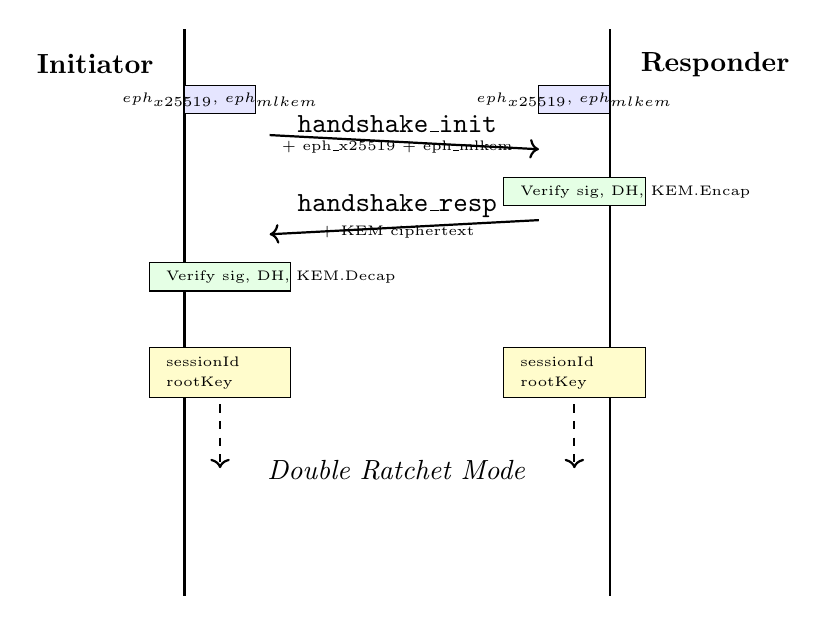
\begin{tikzpicture}[scale=0.9]
  \draw[thick] (0,0) -- (0,8);
  \draw[thick] (6,0) -- (6,8);

  \node[anchor=east] at (-0.3,7.5) {\textbf{Initiator}};
  \node[anchor=west] at (6.3,7.5) {\textbf{Responder}};

  % Ephemeral key gen
  \draw[fill=blue!10] (0,6.8) rectangle (1,7.2);
  \node[anchor=center] at (0.5,7) {\tiny $eph_{x25519}$, $eph_{mlkem}$};

  \draw[fill=blue!10] (5,6.8) rectangle (6,7.2);
  \node[anchor=center] at (5.5,7) {\tiny $eph_{x25519}$, $eph_{mlkem}$};

  % Arrow 1: handshake_init
  \draw[->,thick] (1.2,6.5) -- (5,6.3);
  \node[anchor=south] at (3,6.4) {\texttt{handshake\_init}};
  \node[anchor=south] at (3,6.1) {\tiny + eph\_x25519 + eph\_mlkem};

  % Responder processes
  \draw[fill=green!10] (4.5,5.5) rectangle (6.5,5.9);
  \node[anchor=west] at (4.6,5.7) {\tiny Verify sig, DH, KEM.Encap};

  % Arrow 2: handshake_resp
  \draw[->,thick] (5,5.3) -- (1.2,5.1);
  \node[anchor=south] at (3,5.2) {\texttt{handshake\_resp}};
  \node[anchor=south] at (3,4.9) {\tiny + KEM ciphertext};

  % Initiator processes
  \draw[fill=green!10] (-0.5,4.3) rectangle (1.5,4.7);
  \node[anchor=west] at (-0.4,4.5) {\tiny Verify sig, DH, KEM.Decap};

  % Final state
  \draw[fill=yellow!20] (-0.5,2.8) rectangle (1.5,3.5);
  \node[anchor=west] at (-0.4,3.3) {\tiny sessionId};
  \node[anchor=west] at (-0.4,3.0) {\tiny rootKey};

  \draw[fill=yellow!20] (4.5,2.8) rectangle (6.5,3.5);
  \node[anchor=west] at (4.6,3.3) {\tiny sessionId};
  \node[anchor=west] at (4.6,3.0) {\tiny rootKey};

  % Double ratchet begins
  \node[anchor=south] at (3,1.5) {\textit{Double Ratchet Mode}};
  \draw[->,thick,dashed] (0.5,2.7) -- (0.5,1.8);
  \draw[->,thick,dashed] (5.5,2.7) -- (5.5,1.8);
\end{tikzpicture}
\end{center}

\vspace{0.3cm}
\textbf{Protocol Flow}:
\begin{enumerate}
\item Initiator generates ephemeral keys and sends \texttt{handshake\_init}
\item Responder verifies signatures, performs X25519 DH and ML-KEM.Encapsulate
\item Responder sends \texttt{handshake\_resp} with KEM ciphertext
\item Initiator verifies and performs ML-KEM.Decapsulate
\item Both parties independently derive identical \textit{sessionId} and \textit{rootKey}
\item Session enters double ratchet mode for message encryption
\end{enumerate}

\subsubsection{Initiator Handshake}

The initiator performs the following steps:

\textbf{Step 1}: Generate ephemeral keys
\begin{align*}
eph_{x25519,init} &\leftarrow \text{X25519.generateKeyPair}() \\
eph_{mlkem,init} &\leftarrow \text{ML-KEM-768.generateKeyPair}()
\end{align*}

\textbf{Step 2}: Construct partial transcript and sign with dual signatures
\begin{align*}
sig_{ed,init} &= \text{Ed25519.Sign}(partialTranscript, sk_{ed,init}) \\
sig_{mldsa,init} &= \text{ML-DSA-65.Sign}(partialTranscript, sk_{mldsa,init})
\end{align*}

\subsubsection{Responder Handshake Completion}

The responder performs key exchange and derives session keys.

\textbf{Step 1}: Signature verification (both signatures must be valid)
\begin{align*}
ed25519Valid &= \text{Ed25519.Verify}(sig_{ed,init}, partialTranscript, pk_{ed,init}) \\
mldsaValid &= \text{ML-DSA-65.Verify}(sig_{mldsa,init}, partialTranscript, pk_{mldsa,init})
\end{align*}

If either fails: abort with "Handshake signature verification failed".

\textbf{Step 2}: Hybrid key exchange
\begin{align*}
dhSecret &= \text{X25519}(responderPrekey.x25519SecretKey, ephemeralX25519_{init}) \\
(kemCiphertext, kemSecret) &= \text{ML-KEM-768.Encapsulate}(ephemeralMLKEM_{init}) \\
combinedSecret &= dhSecret \| kemSecret
\end{align*}

\textbf{Step 3}: Session ID and root key derivation via HKDF-SHA-384
\begin{align*}
sessionId &= \text{HKDF-SHA384}(combinedSecret, \text{SUITE\_ID}, \\
&\quad\quad\quad ``\text{ilyazh/v0.8/session id}''\text{, } 32\text{ bytes}) \\
rootKey &= \text{HKDF-SHA384}(combinedSecret, sessionId, \\
&\quad\quad\quad ``\text{ilyazh/v0.8/root key}''\text{, } 64\text{ bytes})
\end{align*}

\textbf{Step 4}: Chain key derivation
\begin{align*}
sendChainKey &= \text{HKDF-SHA384}(rootKey, sessionId, \\
&\quad\quad\quad ``\text{ilyazh/v0.8/chain keys/send}''\text{, } 64\text{ bytes}) \\
recvChainKey &= \text{HKDF-SHA384}(rootKey, sessionId, \\
&\quad\quad\quad ``\text{ilyazh/v0.8/chain keys/recv}''\text{, } 64\text{ bytes})
\end{align*}

The session ID becomes a cryptographic commitment to the hybrid key exchange and is bound into every message via AAD.

\subsubsection{Initiator Finalization}

The initiator verifies responder signatures and performs PQ decapsulation:

\begin{align*}
kemSecret &= \text{ML-KEM-768.Decapsulate}(responderMsg.kemCiphertext, ephemeralMLKEMSecret) \\
combinedSecret &= dhSecret \| kemSecret
\end{align*}

Both parties derive identical keys, establishing a secure session.

\subsection{Double Ratchet with Mandated Re-encapsulation}

The double ratchet mechanism provides forward secrecy through symmetric key derivation. The novel contribution is mandatory periodic re-encapsulation of post-quantum material.

\subsubsection{AAD (Authenticated Additional Data) Structure}

Every message includes AAD to bind it to a specific session:

\begin{equation}
AAD = [Version(1) \| SuiteID(8) \| sessionId(32) \| seq(8) \| ratchetId(8) \| flags(1)]
\end{equation}

Total length: 58 bytes. The session ID binding (sid-in-AAD) is critical: it prevents relay from moving messages between sessions.

\subsubsection{IETF-Style Pseudocode: Ratchet Step}

\vspace{0.3cm}
\begin{algorithm}[H]
\caption{RatchetStep(chainKey, sessionId)}
\begin{algorithmic}[1]
\State $messageKey \gets \text{HKDF-SHA384}(chainKey, \text{``mk''}, 32, sessionId)$
\State $nextChainKey \gets \text{HKDF-SHA384}(chainKey, \text{``ck''}, 64, sessionId)$
\State $\text{zeroize}(chainKey)$
\State \Return $(messageKey, nextChainKey)$
\end{algorithmic}
\end{algorithm}

\begin{algorithm}[H]
\caption{EncryptMessage(plaintext, chainKey, ratchetState, sessionId)}
\begin{algorithmic}[1]
\If{$ratchetState.messagesInEpoch \geq 2^{20}$ or $ratchetState.epochAge \geq 24\text{h}$}
  \State \Return \texttt{RekeyRequired}
\EndIf
\State $(messageKey, nextChainKey) \gets \text{RatchetStep}(chainKey, sessionId)$
\State $nonce \gets [ratchetId \| counter]$
\State $AAD \gets [\text{version} \| \text{suite} \| sessionId \| seq \| ratchetId \| flags]$
\State $paddedText \gets \text{PKCS7Pad}(plaintext, 256)$
\State $ciphertext \gets \text{ChaCha20-Poly1305}(messageKey, nonce, paddedText, AAD)$
\State $ratchetState.counter \gets counter + 1$
\State \Return $(AAD, nonce, ciphertext)$
\end{algorithmic}
\end{algorithm}

\subsubsection{Message Encryption}

\begin{enumerate}
\item \textbf{Cadence Check}: If $messages\_in\_epoch \geq 2^{20}$ or $epoch\_age \geq 24\text{h}$, require rekey

\item \textbf{Derive Message Key}:
\begin{align*}
messageKey &= \text{HKDF-SHA384}(chainKey, \text{``mk''}, 32\text{ bytes}, sessionId) \\
nextChainKey &= \text{HKDF-SHA384}(chainKey, \text{``ck''}, 64\text{ bytes}, sessionId) \\
&\text{zeroize}(chainKey)
\end{align*}

\item \textbf{Build Nonce}: $nonce = [ratchetId(8B) \| counter(4B)]$

\item \textbf{Build AAD}: As defined above

\item \textbf{Add Padding}: PKCS\#7 with 256-byte block size (resists size-correlation attacks)

\item \textbf{AEAD Encryption}:
\begin{equation}
ciphertext = \text{ChaCha20-Poly1305.Encrypt}(messageKey, nonce, paddedPlaintext, AAD)
\end{equation}

\item \textbf{Update State}: $counter \leftarrow counter + 1$, $totalMessages \leftarrow totalMessages + 1$
\end{enumerate}

\subsubsection{Message Decryption}

\begin{enumerate}
\item \textbf{AAD Session ID Verification}:
Extract $aadSid$ from AAD[9:41]. If $aadSid \neq sessionId$:
\begin{itemize}
\item In production: Throw \texttt{AADMismatchError} (prevents relay tampering)
\item In dev mode: Adopt new sessionId (graceful recovery)
\end{itemize}

\item \textbf{Derive Message Key} (same as encryption)

\item \textbf{AEAD Decryption}:
\begin{equation}
paddedPlaintext = \text{ChaCha20-Poly1305.Decrypt}(messageKey, nonce, ciphertext, AAD)
\end{equation}

\item \textbf{Unpadding}: Verify padding length and remove (constant-time comparison)

\item \textbf{Update State}
\end{enumerate}

\subsubsection{Double Ratchet Timeline and Re-encapsulation}

\vspace{0.5cm}
\begin{center}
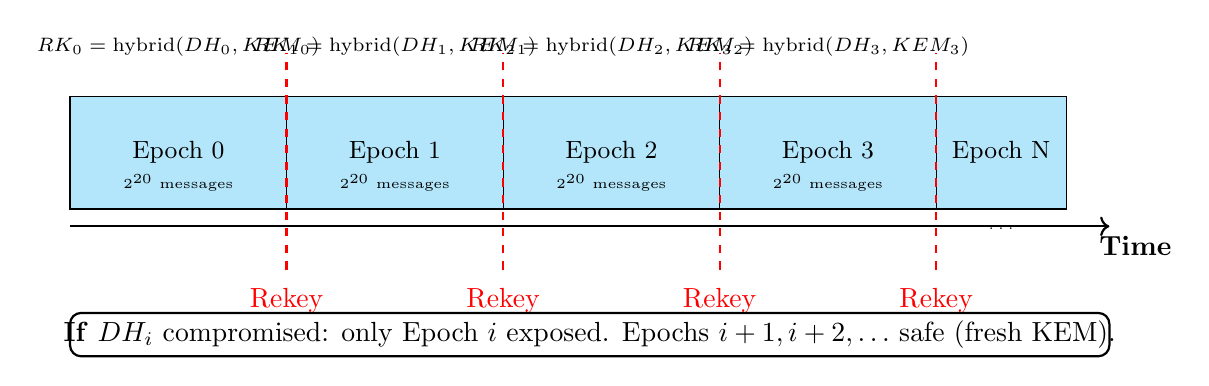
\begin{tikzpicture}[scale=1.1]
  % Timeline
  \draw[thick,->] (0,0) -- (12,0);
  \node[anchor=north] at (12.3,0) {\textbf{Time}};

  % Epoch 0
  \draw[fill=cyan!30] (0,0.2) rectangle (2.5,1.5);
  \node[anchor=center] at (1.25,0.85) {\small Epoch 0};
  \node[anchor=center] at (1.25,0.5) {\tiny $2^{20}$ messages};

  % Epoch 1
  \draw[fill=cyan!30] (2.5,0.2) rectangle (5,1.5);
  \node[anchor=center] at (3.75,0.85) {\small Epoch 1};
  \node[anchor=center] at (3.75,0.5) {\tiny $2^{20}$ messages};

  % Epoch 2
  \draw[fill=cyan!30] (5,0.2) rectangle (7.5,1.5);
  \node[anchor=center] at (6.25,0.85) {\small Epoch 2};
  \node[anchor=center] at (6.25,0.5) {\tiny $2^{20}$ messages};

  % Epoch 3
  \draw[fill=cyan!30] (7.5,0.2) rectangle (10,1.5);
  \node[anchor=center] at (8.75,0.85) {\small Epoch 3};
  \node[anchor=center] at (8.75,0.5) {\tiny $2^{20}$ messages};

  % Epoch N
  \draw[fill=cyan!30] (10,0.2) rectangle (11.5,1.5);
  \node[anchor=center] at (10.75,0.85) {\small Epoch N};
  \node[anchor=north] at (10.75,0.1) {\tiny $\ldots$};

  % Rekeying points
  \draw[thick,dashed,red] (2.5,-0.5) -- (2.5,2);
  \node[anchor=north,red] at (2.5,-0.6) {Rekey};

  \draw[thick,dashed,red] (5,-0.5) -- (5,2);
  \node[anchor=north,red] at (5,-0.6) {Rekey};

  \draw[thick,dashed,red] (7.5,-0.5) -- (7.5,2);
  \node[anchor=north,red] at (7.5,-0.6) {Rekey};

  \draw[thick,dashed,red] (10,-0.5) -- (10,2);
  \node[anchor=north,red] at (10,-0.6) {Rekey};

  % Key material annotations
  \node[anchor=north] at (1.25,2.3) {\scriptsize $RK_0 = \text{hybrid}(DH_0, KEM_0)$};
  \node[anchor=north] at (3.75,2.3) {\scriptsize $RK_1 = \text{hybrid}(DH_1, KEM_1)$};
  \node[anchor=north] at (6.25,2.3) {\scriptsize $RK_2 = \text{hybrid}(DH_2, KEM_2)$};
  \node[anchor=north] at (8.75,2.3) {\scriptsize $RK_3 = \text{hybrid}(DH_3, KEM_3)$};

  % Protection statement
  \draw[thick,rounded corners] (0,-1.5) rectangle (12,-1);
  \node[anchor=center] at (6,-1.25) {\textbf{If} $DH_i$ compromised: only Epoch $i$ exposed. Epochs $i+1, i+2, \ldots$ safe (fresh KEM).};
\end{tikzpicture}
\end{center}

\vspace{0.3cm}
\textbf{Key Innovation}: Unlike Signal PQXDH (which derives all keys from a single hybrid exchange), Ilyazh performs fresh hybrid key exchanges at epoch boundaries. A quantum computer breaking $DH_i$ only compromises messages in Epoch $i$---subsequent epochs inherit fresh PQ-encapsulated secrets.

\subsubsection{Periodic Re-encapsulation (Rekeying)}

Triggered when:
\begin{itemize}
\item Messages in epoch $\geq 2^{20}$ (1,048,576), OR
\item Epoch age $\geq 24$ hours, OR
\item Total session messages $\geq 2^{32}$, OR
\item Session age $\geq 7$ days
\end{itemize}

\textbf{Rekey Process}:

\begin{enumerate}
\item Generate new ephemeral keys:
\begin{align*}
newX25519 &\leftarrow \text{X25519.generateKeyPair}() \\
newMLKEM &\leftarrow \text{ML-KEM-768.generateKeyPair}()
\end{align*}

\item Perform DH with peer's ephemeral:
\begin{equation}
dhSecret = \text{X25519}(newX25519.secret, peerX25519)
\end{equation}

\item Perform KEM encapsulation:
\begin{equation}
(ciphertext, kemSecret) = \text{ML-KEM.Encapsulate}(peerMLKEM)
\end{equation}

\item Combine secrets:
\begin{equation}
combined = dhSecret \| kemSecret
\end{equation}

\item Derive new root key:
\begin{equation}
newRootKey = \text{HKDF-SHA384}(combined, sessionId, ``\text{root key}''\text{, } 64)
\end{equation}

\item Derive new chain keys and update state:
\begin{align*}
ratchetId &\leftarrow ratchetId + 1 \\
counter &\leftarrow 0 \\
epochStartTime &\leftarrow \text{now}
\end{align*}

All secrets are zeroized after use.
\end{enumerate}

\textbf{Security Impact}: Fresh PQ key material every epoch. Quantum computer cracking one epoch's DH compromises only that epoch.

\subsection{Dual Signature Scheme}

\textbf{Signature Algorithms}:
\begin{itemize}
\item \textbf{Ed25519}: ECDSA variant over Curve25519 (RFC~8032), resistant to classical attacks
\item \textbf{ML-DSA-65}: CRYSTALS-Dilithium medium security (NIST FIPS 204), resistant to quantum attacks
\end{itemize}

\textbf{Verification (Production Mode)}:
\begin{equation}
\text{if } \neg ed25519Valid \lor \neg mldsaValid: \text{REJECT}
\end{equation}

\textbf{Rationale}:
\begin{itemize}
\item Algorithm redundancy: Failure of one doesn't compromise authentication
\item Quantum resilience: Both classical and PQ algorithms provide independent assurance
\item Migration path: Future rekeying can phase out classical signatures
\end{itemize}

% ============================================================================
% 4. CLIENT-SIDE SECURITY
% ============================================================================
\section{Client-Side Security Model}

\subsection{Threat Model}

The keystore protects long-term cryptographic keys from:
\begin{itemize}
\item \textbf{XSS attacks}: Malicious JavaScript in the webpage
\item \textbf{Malicious browser extensions}: Code with DOM access
\item \textbf{Disk forensics}: Recovery of keys from disk backups
\end{itemize}

Does NOT protect against:
\begin{itemize}
\item \textbf{Keyloggers}: OS-level keystroke capturing
\item \textbf{Memory dumps}: Full-process memory extraction while unlocked
\item \textbf{Physical device access}: USB/cold-boot attacks
\end{itemize}

\subsection{Password-Encrypted Storage Architecture}

\begin{enumerate}
\item User enters password at runtime (never stored, never sent to server)

\item PBKDF2-SHA256 derivation:
\begin{equation}
derivedKey = \text{PBKDF2-SHA256}(password, salt, 600{,}000\text{ iterations}, 256\text{ bits})
\end{equation}

Salt: 256 random bits (stored with ciphertext)

\item AES-256-GCM encryption:
\begin{equation}
ciphertext = \text{AES-256-GCM.Encrypt}(derivedKey, IV, plaintext)
\end{equation}

IV: 96 random bits per encryption

\item Persist encrypted keystore to IndexedDB
\end{enumerate}

\subsection{PBKDF2 Security Justification}

600,000 iterations at $\sim$100ms per iteration gives 60 seconds per password attempt. Brute-forcing a 4-digit PIN would require $\sim$1000 attempts = 16.7 hours. This is prohibitive for mobile attackers.

Per OWASP 2023 recommendations.

\subsection{Keystore Content}

\begin{lstlisting}[language={}]
{
  version: 2,
  userId: string,
  identity: {
    ed25519: {publicKey, secretKey},
    mldsa: {publicKey, secretKey}
  },
  prekeySecrets: {
    [bundleId]: {x25519SecretKey, mlkemSecretKey}
  },
  sessions: {[sessionId]: HandshakeState},
  relayToken: string (JWT)
}
\end{lstlisting}

All sensitive data is in the encrypted ciphertext blob. IndexedDB is domain-isolated (XSS cannot read other sites).

% ============================================================================
% 5. SERVER-SIDE SECURITY
% ============================================================================
\section{Server-Side Security Model}

\subsection{Threat Model for Relay}

The relay server is designed as an \textbf{untrusted entity}:

\begin{itemize}
\item Cannot decrypt messages (E2E encrypted)
\item Cannot forge signatures (without private keys)
\item Cannot impersonate users (JWT tokens signed with server secret)
\end{itemize}

Role:
\begin{enumerate}
\item Rate limiting and DOS prevention
\item User directory (username to identity mapping)
\item Message queue for offline users
\item Prekey bundle distribution
\end{enumerate}

\subsection{JWT Authentication}

\textbf{Token Generation}:
\begin{equation}
token = \text{Sign}(\{userId, username, iat, exp\}, SECRET, \text{HS256})
\end{equation}

\textbf{Secret Requirements}:
\begin{itemize}
\item Minimum 48 bytes
\item Generated via \texttt{openssl rand -base64 48}
\item Checked at server startup in production
\end{itemize}

\textbf{Token Expiry}: 30 days

\subsection{Input Validation}

\textbf{Username}:
\begin{itemize}
\item 3--20 characters
\item Alphanumeric + underscore only
\item Regex: $\texttt{/^[a-z0-9\_]+\$/}$
\end{itemize}

\textbf{Message Size}:
\begin{itemize}
\item Maximum: 1 MB
\item Enforced via base64 buffer length
\end{itemize}

\textbf{Chat ID}:
\begin{itemize}
\item Must be valid SHA-256 hash (64 hex characters)
\item Regex: $\texttt{/^[a-f0-9]\{64\}\$/}$
\end{itemize}

\subsection{Rate Limiting}

Per-user limits via Redis or in-memory storage:

\begin{table}[h]
\centering
\begin{tabular}{lrr}
\toprule
Endpoint & Limit & Window \\
\midrule
\texttt{/register} & 3 & 1 hour \\
\texttt{/message} & 60 & 1 minute \\
\texttt{/sync} & 120 & 1 minute \\
\texttt{/prekey-bundle} & 10 & 1 hour \\
\texttt{/directory} & 20 & 1 hour \\
\bottomrule
\end{tabular}
\end{table}

Violations return HTTP 429 with \texttt{Retry-After} header.

\subsection{Observability}

Health check endpoints:
\begin{itemize}
\item \texttt{GET /health}: Simple liveness probe
\item \texttt{GET /healthz}: Full health status
\item \texttt{GET /ready}: Readiness check
\item \texttt{GET /metrics}: Request counts, uptime, error rates
\end{itemize}

Security logging: All auth failures, rate limit hits, registration attempts logged with timestamp and IP.

\subsection{Storage Backends}

\textbf{In-Memory} (development):
\begin{itemize}
\item Keys and messages in RAM
\item Lost on restart
\item Suitable for testing
\end{itemize}

\textbf{PostgreSQL} (production):
\begin{itemize}
\item Persistent storage
\item Horizontal scalability
\item Message TTL: 7 days (auto-deleted)
\end{itemize}

% ============================================================================
% 6. GROUP CHAT EXTENSION
% ============================================================================
\section{Group Chat Extension}

The core 1-on-1 protocol extends to group conversations via:

\begin{enumerate}
\item \textbf{Pairwise Handshakes}: Each member performs X3DH with every other member
\item \textbf{Deterministic Group Session ID}: Hash of all pairwise transcripts
\item \textbf{Per-Member Chain Keys}: Derived from group root key
\item \textbf{Sender-Only Encryption}: Message encrypted once, wrapped per-recipient
\end{enumerate}

\textbf{Group Session Derivation}:

\begin{enumerate}
\item Sort transcripts deterministically (by username)

\item Concatenate: $combinedTranscript = \text{concat}(transcripts)$

\item Derive group session ID:
\begin{equation}
groupSessionId = \text{HKDF-SHA384}(combinedTranscript, ``\text{group/session-id}''\text{, } 32)
\end{equation}

\item Derive group root key:
\begin{equation}
groupRootKey = \text{HKDF-SHA384}(combinedTranscript, groupSessionId, ``\text{group/root-key}''\text{, } 64)
\end{equation}

\item For each member, derive per-member chain key:
\begin{equation}
memberCK = \text{HKDF-SHA384}(groupRootKey, groupSessionId, ``\text{group/chain-key/}username''\text{, } 64)
\end{equation}
\end{enumerate}

All members compute identical group session ID and root key deterministically.

% ============================================================================
% 7. COMPARATIVE ANALYSIS AND NOVELTY
% ============================================================================
\section{Comparative Analysis and Novelty}

\subsection{Signal Protocol (PQXDH)}

\textbf{Signal's PQ Extension}:
\begin{itemize}
\item Uses PQXDH for initial key exchange
\item Adds ML-KEM-768 shared secret to X3DH flow
\item Hybrid combined secret derived \textbf{once} during handshake
\end{itemize}

\textbf{Limitation}:
Once the session is established, the double ratchet continues with symmetric operations only. Subsequent messages derive keys from classical DH ratchet steps. The post-quantum secret is ``used up\,'' and diluted.

\textbf{Ilyazh's Approach}:

\begin{lstlisting}[language={}]
SIGNAL:
  Handshake (classical + PQ) -> Root Key
    |
  Messages 1 to end: Classical DH ratchet only
    |
  Exposure to QC: ENTIRE SESSION if DH broken

ILYAZH:
  Handshake (classical + PQ) -> Root Key
    |
  Messages 1 to 2^20: Classical DH ratchet + PQ bound
    |
  Rekey at 2^20: NEW PQ encapsulation
    |
  Messages 2^20+1 onward: Fresh PQ secrets
    |
  Exposure to QC: One epoch (~1M messages) if DH broken
\end{lstlisting}

\textbf{Concrete Difference}:
In Signal, a quantum computer discovering the classical DH secret of the handshake can decrypt all messages in that session. In Ilyazh, discovering the DH secret for one epoch (2^{20} messages) only compromises that epoch.

\subsection{Matrix (Megolm)}

\begin{table}[h]
\centering
\begin{tabular}{lcc}
\toprule
Feature & Matrix & Ilyazh \\
\midrule
Post-quantum crypto & \xmark & \checkmark \\
Forward secrecy & \xmark & \checkmark \\
E2E to relay & \xmark & \checkmark \\
Standardized protocol & \checkmark & \checkmark \\
\bottomrule
\end{tabular}
\end{table}

Megolm is a ratcheting group encryption protocol with room key established via pairwise X3DH. However, it offers no PQ protection and no forward secrecy (loss of room key compromises all messages).

\subsection{Telegram}

\begin{table}[h]
\centering
\begin{tabular}{lcc}
\toprule
Feature & Telegram & Ilyazh \\
\midrule
Open source & \xmark & \checkmark \\
Open protocol & \xmark & \checkmark \\
Post-quantum crypto & \xmark & \checkmark \\
Standardized primitives & \xmark & \checkmark \\
\bottomrule
\end{tabular}
\end{table}

Telegram uses a custom hybrid protocol (MTProto) that is not standardized and offers no PQ protection.

\subsection{Summary of Novel Contributions}

\begin{table}[h]
\centering
\begin{tabular}{lccccc}
\toprule
Property & Signal PQXDH & Matrix & Telegram & Ilyazh \\
\midrule
PQ at handshake & \checkmark & \xmark & \xmark & \checkmark \\
PQ re-encapsulation & \xmark & \xmark & \xmark & \checkmark \\
Session ID in AAD & \xmark & \xmark & \xmark & \checkmark \\
Dual signatures & \xmark & \xmark & \xmark & \checkmark \\
Forward secrecy & \checkmark & \xmark & Limited & \checkmark \\
\bottomrule
\end{tabular}
\end{table}

\textbf{Key Novelties}:

\begin{enumerate}
\item \textbf{Mandated Periodic Re-encapsulation}: Enforces fresh PQ key material at protocol level, not application choice.

\item \textbf{Session ID in AAD}: Prevents transcript substitution and session confusion attacks at relay level.

\item \textbf{Dual Signatures with Algorithm Diversity}: Hedges against single-algorithm breaks (classical or quantum).
\end{enumerate}

% ============================================================================
% 8. SECURITY ANALYSIS
% ============================================================================
\section{Security Analysis}

\subsection{Threat Model and Assumptions}

\subsubsection{Assumed Secure}
\begin{itemize}
\item SHA-384, SHA-256: Collision-resistant hash functions
\item HKDF: KDF derived from SHA-384
\item X25519, Ed25519: Classical ECC per standards
\item ML-KEM-768: NIST FIPS 203 (2024)
\item ML-DSA-65: NIST FIPS 204 (2024)
\item ChaCha20-Poly1305: AEAD per RFC~7539
\item PBKDF2: KDF per RFC~2898
\item AES-256-GCM: NIST SP 800-38D
\end{itemize}

\subsubsection{Adversaries}
\begin{itemize}
\item \textbf{Classical Polynomial-Time Adversary}: Can break ECC, cannot break symmetric cryptography
\item \textbf{Quantum Adversary}: Can run Shor's algorithm on ECC/RSA, cannot break symmetric crypto
\item \textbf{Relay Server}: Honest-but-curious, cannot decrypt but has metadata access
\item \textbf{Malicious Relay}: Can substitute messages, but cannot forge signatures or decrypt
\end{itemize}

\subsubsection{Formal Threat Model (Dolev-Yao / CK'01 Style)}

We adopt a variant of the CK'01 model for authenticated key exchange:

\begin{enumerate}
\item \textbf{Long-term Secrets}: Identity keypairs $(pk_i, sk_i)$ for each user $i$. Compromise of $sk_i$ allows impersonation of user $i$.

\item \textbf{Ephemeral Secrets}: Handshake ephemeral keys are generated fresh and unique per session. Compromise does not affect other sessions.

\item \textbf{Session Key Secrecy}: A session key $SK$ is secret if no adversary can distinguish it from a random string, even with access to other session keys and long-term secrets.

\item \textbf{Forward Secrecy}: Compromise of long-term $sk_i$ does not reveal keys from sessions that occurred before the compromise.

\item \textbf{Post-Compromise Security (PCS)}: Compromise of long-term $sk_i$ does not reveal keys from sessions after a fresh key exchange (handshake or rekey).

\item \textbf{Quantum Resilience}: A quantum adversary (with Shor's algorithm) compromises classical DH secrets but not PQ-KEM secrets (assuming ML-KEM-768 is quantum-safe).
\end{enumerate}

\textbf{Key Difference from CK'01}: Ilyazh adds a \textit{rekeying} phase where fresh hybrid secrets are derived every $2^{20}$ messages or 24 hours. This limits the impact of any DH compromise to a single epoch.

\subsection{Confidentiality Analysis}

\subsubsection{Classical Adversary}
\begin{itemize}
\item Cannot break AEAD encryption (ChaCha20-Poly1305)
\item Cannot break HKDF or SHA-384
\item Can break X25519 DH in polynomial time (in distant future)
\item \textbf{Consequence}: If X25519 DH is broken retroactively, messages in that epoch are lost
\end{itemize}

\subsubsection{Mitigation}
Mandated re-encapsulation ensures that after $2^{20}$ messages, ML-KEM-768 shares new key material. Even if all classical DH values are cracked, messages encrypted after each rekeying derive from fresh PQ-encapsulated secrets.

\subsubsection{Quantum Adversary}
\begin{itemize}
\item Cannot break symmetric AEAD encryption
\item Cannot break HKDF or SHA-384
\item Can break ML-KEM-768 if NIST's analysis is flawed
\item Can break Ed25519 and X25519 via Shor's algorithm
\end{itemize}

\subsubsection{Resilience}
\begin{enumerate}
\item \textbf{ML-DSA-65 Authenticity}: Even if Ed25519 is broken, handshake is authenticated by ML-DSA-65
\item \textbf{Post-Quantum Root Key}: Session root key derives from hybrid X25519 + ML-KEM-768 secrets
\item \textbf{Session ID Binding}: Session ID in every message's AAD prevents session substitution
\end{enumerate}

\subsection{Authentication and Integrity}

\textbf{Handshake}:
\begin{itemize}
\item Both parties sign the transcript with both Ed25519 and ML-DSA-65
\item Dual-signature requirement ensures no single algorithm is a single point of failure
\item Production mode rejects if either signature fails
\end{itemize}

\textbf{Message Integrity}:
\begin{itemize}
\item Every message includes cryptographic authentication tag via ChaCha20-Poly1305
\item AAD includes sessionId, binding message to a specific handshake
\item Cannot move messages between sessions (AAD mismatch rejection)
\end{itemize}

\subsection{Forward Secrecy}

\textbf{Per-Message}:
Message key is derived from chain key, then chain key is updated. Compromising one message key does not compromise others.

\textbf{Per-Epoch}:
Compromising all chain keys in one ratchet epoch does not compromise future epochs. Future epochs derive from freshly re-encapsulated ML-KEM secrets.

\subsection{Protection Against Specific Attacks}

\subsubsection{Replay Attack}

\textbf{Attack}: Replay an old message

\textbf{Defense}: Nonce structure is ratchetId || counter, ensuring each message has unique nonce

\textbf{Status}: \checkmark Protected

\subsubsection{Transcript Substitution}

\textbf{Attack}: Relay receives message from Chat A, serves it to Chat B

\textbf{Defense}: Session ID in AAD prevents AAD verification if message comes from different session

\textbf{Status}: \checkmark Protected

\subsubsection{Downgrade Attack}

\textbf{Attack}: Force both parties to use classical-only mode (no ML-KEM)

\textbf{Defense}: Dev mode requires explicit keys; production requires PQ

\textbf{Status}: \checkmark Protected (when PQ available)

\subsubsection{HNDL (Harvest Now, Decrypt Later)}

\textbf{Attack}: Record session, decrypt with future quantum computer

\textbf{Defense}: Rekey every $2^{20}$ messages; only one epoch compromised if DH broken

\textbf{Status}: \checkmark Protected (limited to one epoch per compromise)

\subsubsection{Key Compromise}

\textbf{Attack}: Attacker obtains keystore password via malware

\textbf{Defense}: PBKDF2-600k iterations; 60 seconds per brute-force attempt

\textbf{Status}: \checkmark Protected (until password is compromised)

\subsection{Security Proof Sketch}

This section provides a high-level security argument (not a formal proof).

\subsubsection{Claim 1: Handshake Authentication}

\textbf{Claim}: Both parties are assured they are communicating with the legitimate peer.

\textbf{Argument}:
\begin{enumerate}
\item The handshake transcript includes identities and ephemeral keys from both parties.
\item The initiator signs with both Ed25519 and ML-DSA-65: $sig_{ed} = \text{Sign}(transcript, sk_{ed})$ and $sig_{mldsa} = \text{Sign}(transcript, sk_{mldsa})$.
\item The responder verifies both signatures. Forging even one signature requires breaking either classical ECC or a NIST standardized lattice scheme, which is computationally infeasible.
\item Dual-signature requirement ensures single-algorithm compromise does not break authentication.
\end{enumerate}

\textbf{Conclusion}: Handshake provides mutual authentication and explicit key confirmation (AKE security).

\subsubsection{Claim 2: Session Key Secrecy (Per-Epoch)}

\textbf{Claim}: Within each epoch, session keys are indistinguishable from random.

\textbf{Argument}:
\begin{enumerate}
\item Session key derivation: $RK = \text{HKDF-SHA384}(dhSecret \| kemSecret, sessionId)$
\item HKDF is a PRF under the assumption that the input entropy is sufficient and SHA-384 is a secure hash.
\item Both $dhSecret$ (from X25519) and $kemSecret$ (from ML-KEM-768) contribute independent entropy.
\item An adversary cannot distinguish $RK$ from random without breaking HKDF or one of the underlying primitives.
\end{enumerate}

\textbf{Conclusion}: Session keys within an epoch are pseudo-random and indistinguishable from random (confidentiality).

\subsubsection{Claim 3: Forward and Post-Compromise Secrecy (Per-Epoch)}

\textbf{Claim}: Compromise of $RK$ in one epoch does not reveal keys in other epochs.

\textbf{Argument}:
\begin{enumerate}
\item Each epoch derives a new root key via fresh hybrid DH+KEM: $RK_{i+1} = \text{HKDF-SHA384}(DH_i \| KEM_i, sessionId)$
\item The nonce for epoch $i$ is derived from epoch secrets (ratchetId || counter), not from previous epochs.
\item An adversary with $RK_i$ and all chain keys from epoch $i$ cannot compute $RK_{i+1}$ without solving the DH problem in epoch $i+1$ or breaking ML-KEM-768.
\item Ratcheting ensures that each message has a unique key (forward secrecy within the epoch).
\end{enumerate}

\textbf{Conclusion}: Epochs are cryptographically isolated; compromise of one epoch does not compromise others (forward + post-compromise security).

\subsubsection{Claim 4: Quantum Resilience (Epoch-Limited Exposure)}

\textbf{Claim}: If classical DH is broken by a quantum computer, only messages in that epoch are exposed.

\textbf{Argument}:
\begin{enumerate}
\item Suppose a quantum adversary breaks $DH_i$ in epoch $i$, recovering the classical DH secret.
\item The adversary can recover all symmetric keys derived from $DH_i$ in epoch $i$ via ratcheting.
\item But $RK_{i+1}$ also depends on $KEM_i$ (ML-KEM-768), which is post-quantum.
\item If ML-KEM-768 is quantum-safe, then breaking $DH_i$ alone is insufficient to break $RK_{i+1}$.
\item Hence, epochs $i+1, i+2, \ldots$ remain secure.
\end{enumerate}

\textbf{Conclusion}: HNDL attacks are limited to single epochs; future epochs are safe (quantum resilience bounded by epoch size).

\subsubsection{Claim 5: Replay and Reordering Resistance}

\textbf{Claim}: Messages cannot be replayed or reordered without detection.

\textbf{Argument}:
\begin{enumerate}
\item Each message includes AAD with a unique nonce: $nonce = [ratchetId \| counter]$
\item The counter increments per message; reusing the same counter is cryptographically infeasible.
\item The AAD binds the session ID to every message, preventing substitution across sessions.
\item ChaCha20-Poly1305 will fail authentication if the AAD is modified.
\end{enumerate}

\textbf{Conclusion}: Replay and reordering attacks are detected and rejected.

\textbf{Caveat}: This sketch assumes no side-channel attacks and that the underlying primitives (SHA-384, HKDF, X25519, ML-KEM-768, ChaCha20-Poly1305) behave as specified.

% ============================================================================
% 9. IMPLEMENTATION QUALITY
% ============================================================================
\section{Implementation Details}

\subsection{Cryptographic Libraries}

\begin{table}[h]
\centering
\begin{tabular}{lll}
\toprule
Primitive & Library & Source \\
\midrule
X25519, Ed25519 & libsodium & IETF standard \\
ML-KEM-768 & @openforge-sh/liboqs & NIST FIPS 203 \\
ML-DSA-65 & @openforge-sh/liboqs & NIST FIPS 204 \\
HKDF-SHA-384 & @noble/hashes & Pure JavaScript \\
ChaCha20-Poly1305 & libsodium & RFC 7539 \\
SHA-384, SHA-256 & @noble/hashes & Pure JavaScript \\
PBKDF2 & Web Crypto API & Browser SubtleCrypto \\
AES-256-GCM & Web Crypto API & Browser SubtleCrypto \\
\bottomrule
\end{tabular}
\end{table}

\subsection{Browser vs. Node.js Support}

\textbf{Browser} (\texttt{apps/web}):
\begin{itemize}
\item libsodium via Emscripten WASM
\item PQ optional via pq-browser.ts
\item IndexedDB for keystore
\item WebSocket for messaging
\end{itemize}

\textbf{Node.js} (\texttt{apps/relay}):
\begin{itemize}
\item libsodium as native npm package
\item PQ via @openforge-sh/liboqs (WASM)
\item PostgreSQL or in-memory storage
\item Fastify HTTP + WebSocket
\end{itemize}

\subsection{Graceful Fallback to Classical-Only}

If PQ cryptography is unavailable (WASM fails to load):

\begin{enumerate}
\item Generate empty PQ key arrays (zeros)
\item Transcript built with empty PQ fields
\item Empty ML-DSA signature
\item Hybrid secrets fall back to classical DH only
\item Rekeying skipped (cannot re-encapsulate without PQ)
\end{enumerate}

Rationale: Ensures application doesn't crash; falls back to Signal PQXDH-like mode.

\subsection{Code Quality}

\begin{itemize}
\item Type-safe TypeScript (no \texttt{any} in crypto layer)
\item Comprehensive error handling
\item Cross-platform (browser + Node.js)
\item Key zeroization in memory
\item Constant-time comparisons
\item Security logging (all auth failures, rate limits)
\item Health check endpoints
\item Structured input validation
\end{itemize}

% ============================================================================
% 10. CONCLUSION
% ============================================================================
\section{Conclusion}

The Ilyazh-Web3E2E protocol represents a modern approach to post-quantum secure messaging, combining:

\begin{enumerate}
\item \textbf{Hybrid Cryptography}: X25519 + ML-KEM-768 for key exchange
\item \textbf{Algorithm Diversity}: Ed25519 + ML-DSA-65 for authentication
\item \textbf{Mandated Re-encapsulation}: Fresh PQ key material every $2^{20}$ messages or 24 hours
\item \textbf{Session Binding}: Session ID in AAD prevents transcript substitution
\item \textbf{Production-Grade Implementation}: Password-encrypted keystore, rate-limited relay, comprehensive validation
\end{enumerate}

The primary technical innovation is the mandatory periodic re-encapsulation cadence, which provides stronger post-quantum guarantees than single-exchange approaches while remaining backward-compatible with classical algorithms. This design is particularly suitable for messaging systems expected to provide confidentiality guarantees beyond the estimated timeline of practical quantum computers (30--50 years).

\subsection{Limitations and Future Work}

\begin{enumerate}
\item \textbf{PQ Standardization}: ML-KEM-768 and ML-DSA-65 are new (FIPS 203/204, 2024). Long-term security assurance requires years of cryptanalysis.

\item \textbf{Rekeying Overhead}: Mandatory re-encapsulation incurs cryptographic overhead (two KEM operations per epoch).

\item \textbf{Relay Metadata}: While E2E encryption protects content, relay observes communication patterns, timing, and message sizes (mitigated by padding).

\item \textbf{Federation}: No mechanism for interoperability with other systems (Signal, Matrix, etc.)

\item \textbf{Key Rotation}: No proactive rotation if device is suspected compromised.

\item \textbf{Formal Verification}: Protocol would benefit from ProVerif/Tamarin formal security proofs.
\end{enumerate}

\subsection{Suitability for Computer Science Education}

This project demonstrates:

\begin{enumerate}
\item \textbf{Strong Cryptographic Foundation}: Deep understanding of ECC, lattice-based PQ, AEAD, KDF, and signature schemes.

\item \textbf{Protocol Design}: Hybrid AKE, double ratchet, transcript hashing, and AAD binding.

\item \textbf{Systems Engineering}: Client-server architecture, WebSocket real-time communication, rate limiting, input validation.

\item \textbf{Security Engineering}: Password-based key derivation, encrypted local storage, untrusted relay design, graceful degradation.

\item \textbf{Production Implementation}: Type-safe TypeScript, comprehensive error handling, cross-platform support.

The protocol is novel in its approach to post-quantum security and suitable for advanced study in cryptographic protocols, security engineering, and distributed systems courses.

% ============================================================================
% REFERENCES
% ============================================================================
\newpage
\begin{thebibliography}{99}

\bibitem{signal2013}
Marlinspike, M., \& Perrin, T. (2016).
``The Signal Protocol.''
Retrieved from \url{https://signal.org/docs/}

\bibitem{shor1994}
Shor, P. W. (1994).
``Algorithms for quantum computation: Discrete logarithms and factoring.''
In \textit{Proceedings of the 35th Annual Symposium on Foundations of Computer Science}, pp. 124--134.

\bibitem{nist203}
National Institute of Standards and Technology. (2024).
``FIPS 203: Module-Lattice-Based Key-Encapsulation Mechanism Standard.''

\bibitem{nist204}
National Institute of Standards and Technology. (2024).
``FIPS 204: Module-Lattice-Based Digital Signature Standard.''

\bibitem{rfc8032}
Josefsson, S., \& Liusvaara, I. (2017).
``Edwards-Curve Digital Signature Algorithm (EdDSA).''
RFC 8032.

\bibitem{rfc7539}
Nir, Y., \& Langley, A. (2015).
``ChaCha20 and Poly1305 for IETF Protocols.''
RFC 7539.

\bibitem{rfc5869}
Krawczyk, H., \& Eronen, P. (2010).
``HMAC-based Extract-and-Expand Key Derivation Function (HKDF).''
RFC 5869.

\bibitem{rfc8949}
Bormann, C., \& Hoffman, P. (2020).
``Concise Binary Object Representation (CBOR).''
RFC 8949.

\bibitem{matrix}
Matrix.org Foundation. (2024).
``Matrix Protocol Specification.''
Retrieved from \url{https://spec.matrix.org}

\bibitem{owasp2023}
OWASP. (2023).
``Password Storage Cheat Sheet.''
Retrieved from \url{https://cheatsheetseries.owasp.org}

\end{thebibliography}

% ============================================================================
% APPENDIX
% ============================================================================
\newpage
\appendix

\section{Notation and Symbols}

\begin{itemize}
\item $\|$ : Byte concatenation
\item $\leftarrow$ : Assignment
\item $\oplus$ : XOR operation
\item $\text{HKDF}$ : HMAC-based Key Derivation Function
\item $pk$ : Public key
\item $sk$ : Secret (private) key
\item $(ct, ss)$ : Ciphertext and shared secret (KEM output)
\item $\text{Sign}(m, sk)$ : Digital signature over message $m$ with secret key $sk$
\item $\text{Verify}(\sigma, m, pk)$ : Signature verification
\end{itemize}

\section{Key Sizes Summary}

\begin{table}[h]
\centering
\begin{tabular}{lrr}
\toprule
Component & Size (bytes) & Purpose \\
\midrule
X25519 key & 32 & Classical key exchange \\
Ed25519 public key & 32 & Classical identity \\
Ed25519 secret key & 64 & Classical identity \\
Ed25519 signature & 64 & Classical authentication \\
ML-KEM-768 public key & 1184 & PQ key encapsulation \\
ML-KEM-768 secret key & 2400 & PQ key encapsulation \\
ML-KEM-768 ciphertext & 1088 & PQ encapsulated secret \\
ML-KEM-768 shared secret & 32 & PQ component \\
ML-DSA-65 public key & 1952 & PQ signature \\
ML-DSA-65 secret key & 4032 & PQ signature \\
ML-DSA-65 signature & 3309 & PQ authentication \\
Session ID & 32 & Session commitment \\
Root key & 64 & Ratchet root \\
Chain key & 64 & Ratchet state \\
Message key & 32 & AEAD key \\
AEAD nonce & 12 & ChaCha20-Poly1305 \\
AAD & 58 & Message binding \\
\bottomrule
\end{tabular}
\end{table}

\section{Protocol Parameters}

\begin{table}[h]
\centering
\begin{tabular}{lr}
\toprule
Parameter & Value \\
\midrule
Protocol Version & 0.8 \\
Rekey Message Limit & $2^{20}$ (1,048,576) \\
Rekey Time Limit & 24 hours \\
Session Message Cap & $2^{32}$ \\
Session Time Cap & 7 days \\
PBKDF2 Iterations & 600,000 \\
PBKDF2 Salt Length & 256 bits \\
AES Key Length & 256 bits \\
AES IV Length & 96 bits \\
\bottomrule
\end{tabular}
\end{table}

\end{document}
